\documentclass{jarticle}
\usepackage[dvipdfmx]{graphicx}
\usepackage{here}
\usepackage{listings,jlisting} %日本語のコメントアウトをする場合jlistingが必要
%ここからソースコードの表示に関する設定
\lstset{
	basicstyle={\ttfamily},
		identifierstyle={\small},
		commentstyle={\smallitshape},
		keywordstyle={\small\bfseries},
		ndkeywordstyle={\small},
		stringstyle={\small\ttfamily},
		frame={tb},
		breaklines=true,
		columns=[l]{fullflexible},
		numbers=left,
		xrightmargin=0zw,
		xleftmargin=3zw,
		numberstyle={\scriptsize},
		stepnumber=1,
		numbersep=1zw,
		lineskip=-0.5ex
}
\title{ソフトウェア設計及び実験\\
	第4回レポート}
	\author{6119019056 山口力也}
	\date{2019/05/07日提出}


	\begin{document}
	\maketitle
	\section{静止画に対する画像処理}
	image_cv.cを参考に,画像の左半分の領域のみ色を変換し,表示させるプログラムを作成せよ.
	\subsection{実験結果(プログラム)}
	以下\ref{code:cvkadai01}にソースコードを示す.
	\begin{lstlisting}[caption = 画像を左半分のみ色を変換するプログラム,label=code:cvkadai01]
	/*
	 **
	 *****************************************************************************
	 **
	 ** Project     : OpenCV sample project
	 ** Module      : image_cv.c
	 ** Description : OpenCVによる画像の読み込み(カラープレーンの置き換え)
	 **
	 ** Version : Date:          Author:       Comment:
	 **     1.0   2011/09/16(金) Akinori Tsuji Creation
	 *****************************************************************************
	 **
	 */
	/*________ INCLUDES _______________________________________________________*/
#include <stdio.h>
#include <opencv2/imgproc/imgproc_c.h>
#include <opencv2/highgui/highgui_c.h>

	/*________ MACROS _________________________________________________________*/
	/*________ DEFINITIONS ____________________________________________________*/
#define CONVERT_RGB

	/*________ VARIABLES ______________________________________________________*/
	/*________ LOCAL-FUNCTION PROTOTYPES ______________________________________*/
	/*________ LOCAL-FUNCTIONS ________________________________________________*/

	/*________ MAIN-FUNCTION __________________________________________________*/

int main(int argc, char **argv)
{
	int x, y;
	uchar p[3];
	IplImage *img;
	img = cvLoadImage("test.jpg", CV_LOAD_IMAGE_COLOR);
	if (img == NULL) {
		fprintf(stderr, "*Error* cannot open test.jpg\n");
		return -1;
	}


#ifdef CONVERT_RGB
	for (y = 0; y < img->height; y++) {
		for (x = 0; x < img->width; x++) {
			p[0] = img->imageData[img->widthStep * y + x * 3];	// B
			p[1] = img->imageData[img->widthStep * y + x * 3 + 1];	// G
			p[2] = img->imageData[img->widthStep * y + x * 3 + 2];	// R

			// Image Processing
		}
	}
	for (y = 0; y < img->height; y++) {
		for (x = img->width/2; x < img->width; x++) {

			img->imageData[img->widthStep * y + x * 3] =
				cvRound(p[0] * 1.0);
			img->imageData[img->widthStep * y + x * 3 + 1] =
				cvRound(p[1] * 1.0);
			img->imageData[img->widthStep * y + x * 3 + 2] =
				cvRound(p[2] * 1.0);
		}
	}
#endif

	cvNamedWindow("Image", CV_WINDOW_AUTOSIZE);
	cvShowImage("Image", img);
	cvWaitKey(0);

	cvDestroyWindow("Image");
	cvReleaseImage(&img);

	return 0;
}
\end{lstlisting}
Image ProcessingのRGBを戻す部分で,for文の条件を変更し,画面左半分のみを描画するようにした.
\subsection{実験結果(画像)}
以下\ref{fig:cvkadai01}に結果画像を示す.

\begin{figure}[H]
\begin{center}
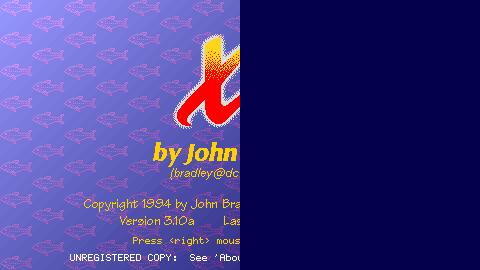
\includegraphics[width=7.0cm]{cv_kadai01/image.png}
\caption{画面左半分のみ色を変換した結果}
\label{fig:cvkadai01}
\end{center}
\end{figure}


\section{カメラを用いた動画に対するテンプレートマッチング}
video_cvを参考にカメラから取得した画像におけるテンプレートマッチングを実現するプログラムを作成せよ.また,テンプレートマッチングを実施した結果について成功例,失敗例を示せ.また,失敗例について,なぜ失敗したのか考察せよ.なお,カラー画像に加え,2値化画像について示せ.
\subsection{実験結果}

以下\ref{code:cvkadai02}にソースコードを示す.
\begin{lstlisting}[caption = 動画に対するテンプレートマッチング,label=code:cvkadai02]
/*
 **
 *****************************************************************************
 **
 ** Project     : OpenCV sample program
 ** Module      : video_cv.c
 ** Description : OpenCV によるUSBカメラ使用
 ** Version : Date:          Author:       Comment:
 **     1.0   2011/09/16(金) Akinori Tsuji Creation
 *****************************************************************************
 **
 */

/*________ INCLUDES _______________________________________________________*/
#include <stdio.h>
#include <opencv2/core/core_c.h>
#include <opencv2/imgproc/imgproc_c.h>
#include <opencv2/highgui/highgui_c.h>

/*________ MACROS _________________________________________________________*/
/*________ DEFINITIONS ____________________________________________________*/
#define CV_DISP_WIDTH   320 // 画面サイズ(横)
#define CV_DISP_HEIGHT  240 // 画面サイズ(縦)
#define THRESHOLD	127     //	2値化の際の閾値
#define THRESHOLD_MAX_VALUE	255     //	2値化の際に使用する最大値
#define LINE_THICKNESS	1	//	線の太さ
#define	LINE_TYPE	8		//	線の種類
#define SHIFT	0			//	座標の小数点以下の桁を表すビット数



/*________ VARIABLES ______________________________________________________*/
/*________ LOCAL-FUNCTION PROTOTYPES ______________________________________*/
/*________ LOCAL-FUNCTIONS ________________________________________________*/

/*________ MAIN-FUNCTION __________________________________________________*/

int main(int argc, char **argv)
{
	CvCapture *capture = 0;
	IplImage *frame = 0;
	double w = CV_DISP_WIDTH, h = CV_DISP_HEIGHT;
	int ckey;
	char windowNameTemplate[] = "Template";			//	テンプレート画像を表示するウィンドウの名前
	char windowNameBinaryTemplate[] = "BinaryTemplate";	//2値化テンプレート画像を表示するウィンドウの名前
	CvPoint minLocation;	//	相違度が最小になる場所

	//	画像を読み込む
	IplImage *templateImage = cvLoadImage( "template.png", CV_LOAD_IMAGE_ANYDEPTH | CV_LOAD_IMAGE_ANYCOLOR );

	if ( templateImage == NULL ){
		//	画像が見つからなかった場合
		printf( "画像が見つかりません\n" );
		return -1;
	}
	//	テンプレート画像をグレースケール化した画像用IplImage	
	IplImage *templateGrayImage = cvCreateImage( cvGetSize(templateImage), IPL_DEPTH_8U, 1 );
	//	テンプレート画像を2値化した画像用IplImage		
	IplImage *templateBinaryImage = cvCreateImage( cvGetSize(templateImage), IPL_DEPTH_8U, 1 );
	//	BGRからグレースケールに変換する
	cvCvtColor( templateImage, templateGrayImage, CV_BGR2GRAY );
	//	グレースケールから2値に変換する
	cvThreshold( templateGrayImage, templateBinaryImage, THRESHOLD, THRESHOLD_MAX_VALUE, CV_THRESH_BINARY );
	// カメラのオープン(/dev/video0)
	capture = cvCreateCameraCapture(0);
	if (capture == NULL) {
		fprintf(stderr, "*Error* cannot open /dev/video0\n");
		return -1;
	}

	// キャプチャサイズの設定
	cvSetCaptureProperty(capture, CV_CAP_PROP_FRAME_WIDTH, w);
	cvSetCaptureProperty(capture, CV_CAP_PROP_FRAME_HEIGHT, h);
	// ウィンドウを生成
	cvNamedWindow("Capture", CV_WINDOW_AUTOSIZE);
	cvNamedWindow("binaryCapture",CV_WINDOW_AUTOSIZE);
	cvNamedWindow( windowNameTemplate, CV_WINDOW_AUTOSIZE);
	cvNamedWindow( windowNameBinaryTemplate,CV_WINDOW_AUTOSIZE);

	cvShowImage( windowNameTemplate,templateImage);
	cvShowImage( windowNameBinaryTemplate,templateBinaryImage);
	// カメラからフレームをキャプチャ
	while (1) {
		frame = cvQueryFrame(capture);

		//	元画像をグレースケール化した画像用IplImage
		IplImage *sourceGrayImage = cvCreateImage( cvGetSize(frame),IPL_DEPTH_8U,1);
		//	元画像を2値化した画像用IplImage	
		IplImage *sourceBinaryImage = cvCreateImage( cvGetSize(frame),IPL_DEPTH_8U,1);
		//	相違度マップ画像用IplImage
		IplImage *differenceMapImage = cvCreateImage( cvSize( frame->width - templateImage->width + 1, frame->height - templateImage->height + 1 ), IPL_DEPTH_32F, 1 );


		//	BGRからグレースケールに変換する
		cvCvtColor ( frame,sourceGrayImage,CV_BGR2GRAY );
		//	グレースケールから2値に変換する
		cvThreshold( sourceGrayImage, sourceBinaryImage, THRESHOLD, THRESHOLD_MAX_VALUE, CV_THRESH_BINARY );
		//	テンプレートマッチングを行う
		cvMatchTemplate( sourceBinaryImage, templateBinaryImage, differenceMapImage, CV_TM_SQDIFF );
		//	テンプレートが元画像のどの部分にあるのかという情報を得る
		cvMinMaxLoc( differenceMapImage, NULL, NULL, &minLocation, NULL, NULL );

		//	一致する場所を元画像に四角で描く
		cvRectangle(
				frame,
				minLocation,
				cvPoint( minLocation.x + templateImage->width, minLocation.y + templateImage->height ),
				CV_RGB( 255, 0, 0 ),
				LINE_THICKNESS,
				LINE_TYPE,
				SHIFT
				);
		//キャプチャ映像の表示
		cvShowImage("Capture", frame);
		// 2値化の映像を表示
		cvShowImage("binaryCapture",sourceBinaryImage);


		ckey = cvWaitKey(10);
		cvReleaseImage(&sourceBinaryImage);
		cvReleaseImage(&sourceGrayImage);
		cvReleaseImage(&differenceMapImage);
		if ((ckey & 0xff) == '\x1b') {
			printf("Exiting ...\n");
			cvSaveImage("image.png",frame,0);
			break; // エスケープキーで終了
		}
	}

	//メモリを解放する
	cvReleaseImage(&templateImage);
	cvReleaseImage(&templateGrayImage);
	cvReleaseImage(&templateBinaryImage);
	cvReleaseCapture(&capture);

	//windowを閉じる
	cvDestroyWindow("Capture");
	cvDestroyWindow("binaryCapture");
	cvDestroyWindow(windowNameTemplate);
	cvDestroyWindow(windowNameBinaryTemplate);
	return 0;
}
\end{lstlisting}

また,以下図\ref{fig:cvkadai02-success-color},図\ref{fig:cvkadai02-success-mono}にテンプレートマッチング成功の一例を示す.


\begin{figure}[H]
\begin{center}
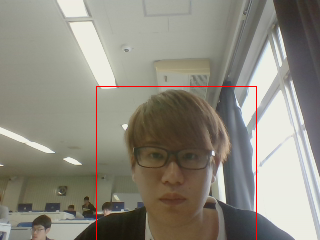
\includegraphics[width=7.0cm]{cv_kadai02/success-color.png}
\caption{テンプレートマッチング成功の一例(カラー)}
\label{fig:cvkadai02-success-color}
\end{center}
\end{figure}

\begin{figure}[H]
\begin{center}
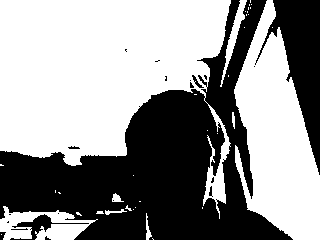
\includegraphics[width=7.0cm]{cv_kadai02/success-mono.png}
\caption{テンプレートマッチング成功の一例(2値化)}
\label{fig:cvkadai02-success-mono}
\end{center}
\end{figure}


以下図\ref{fig:cvkadai02-fail-color},図\ref{fig:cvkadai02-fail-mono}にテンプレートマッチング失敗の一例を示す.


\begin{figure}[H]
\begin{center}
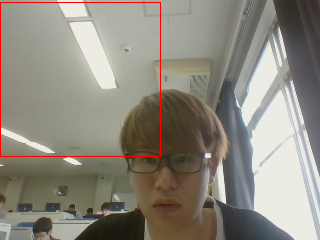
\includegraphics[width=7.0cm]{cv_kadai02/fail-color.png}
\caption{テンプレートマッチング失敗の一例(カラー)}
\label{fig:cvkadai02-fail-color}
\end{center}
\end{figure}

\begin{figure}[H]
\begin{center}
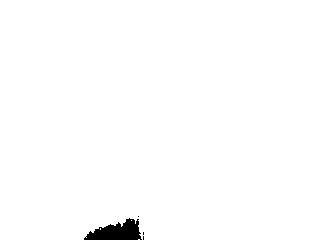
\includegraphics[width=7.0cm]{cv_kadai02/fail-mono.png}
\caption{テンプレートマッチング失敗の一例カラ(2値化)}
\label{fig:cvkadai02-fail-mono}
\end{center}
\end{figure}

\subsection{考察}
実験から失敗するときは2値化する時の閾値が適切でないときであると思われる.閾値が低すぎると2値化した時,黒色となる部分が多すぎてテンプレート画像の特徴を抽出できない.同様に閾値が高すぎると白色となる部分が多すぎてテンプレート画像の特徴を抽出できない.2値化する時の値は0~255であるので中央の127を閾値に設定すると比較的良い精度でテンプレートマッチングをできると思われる.

\section{画像の平滑化}
画像の平滑化とは何か調べて述べよ.また,cvSmooth関数を用いてテンプレート作成用画像を平滑化するプログラムを作成し,平滑化した結果が原画像と比べてどのような画像特性となっているか述べよ.

\subsection{画像の平滑化}
画像の平滑化とは,注目画素の近傍の画素の濃度値の平均を注目画素の新しい濃度値とする方法である.これにより,ごましおノイズのような高い周波数成分のノイズを除去できる.しかしながら,雑音を多く含むような画像では完全に雑音を除去することはできない.
\subsection{平滑化プログラム}
以下ソースコード\ref{code:cvkadai03}にテンプレート作成用画像を平滑化するプログラムを示す.ここで,フィルターはガウシアンフィルタを用いた.
\begin{lstlisting}[caption = 動画に対するテンプレートマッチング,label=code:cvkadai02]
	//インクルード
#include <stdio.h>
#include <opencv2/core/core_c.h>
#include <opencv2/imgproc/imgproc_c.h>
#include <opencv2/highgui/highgui_c.h>

	int main( int argc, char **argv ) {

		char windowNameInputImage[] = "Input";
		char windowNameOutputImage[] = "Output";
		IplImage *inputImage,*outputImage;

		//画像を読み込む
		//入力用と出力用のIplImageを作成
		inputImage = cvLoadImage("lena.png", CV_LOAD_IMAGE_ANYDEPTH | CV_LOAD_IMAGE_ANYCOLOR );
		if ( inputImage== NULL) {
			//	画像が見つからなかった場合
			printf( "画像が見つかりません\n" );
			return -1;
		}
		outputImage =cvCloneImage(inputImage);

		//平滑化フィルタをかける 
		cvSmooth( inputImage ,outputImage,CV_GAUSSIAN,1,0,0,0);

		//ウィンドウを作成
		cvNamedWindow( windowNameInputImage,CV_WINDOW_AUTOSIZE );
		cvNamedWindow( windowNameOutputImage,CV_WINDOW_AUTOSIZE );

		//画像を表示する
		cvShowImage( windowNameInputImage, inputImage);
		cvShowImage( windowNameOutputImage, outputImage);

		//	キー入力を待つ
		cvWaitKey(0);

		//	画像を保存する
		cvSaveImage( "output.bmp", outputImage, 0 );
		cvReleaseImage( &inputImage);
		cvReleaseImage( &outputImage);
		//	ウィンドウを破棄する
		cvDestroyWindow(windowNameInputImage);
		cvDestroyWindow(windowNameOutputImage);

		return 0;
	}
\end{lstlisting}

\subsection{平滑化の特性}
原画像と比べてガウシアンフィルタをかけた時はノイズのようなものが少なくなり,少しぼやけた画像となった.ガウシアンフィルタは注目画素からの距離に応じて近傍の画素値に重みをかける操作を行なっているため,画素の特徴になりえる大きな値は抽出され,ノイズのような小さな値は削除されたためこのような結果になったと考えられる.
\section{デバイスについて}
ソフト実験で利用可能なデバイスの中から1つデバイスを選択し,そのデバイスを用いたゲームを考えて,自分のアイデアをまとめよ.ゲームの概要がわかる図も入れよ.

デバイスとしてはWiiリモコンを選択した.
\subsection{デバイスの特徴と周辺ライブラリ}
WiiリモコンはBluetoothを使用して通信しており,そのためpcでも使うことができる.
そのライブラリとして,「WiimoteLib」というライブラリが用意されている.
必要なものをダウンロードしたあと,"import WiimoteLib"とコードに書くとimportして使うことができる.
Wiiリモコンには

\begin{itemize}

\item バイブレーダ
\item LED
\item ボタン
\item 加速度センサ
\item 赤外線センサ

\end{itemize}
が搭載されており,それぞれを用いてゲームなどを開発できる.

\subsection{ゲーム内容}

自分が作ろうと思うゲームは「イライラ棒」である. Wiiリモコンでのゲーム開発は初めてであるため比較的簡単なものにした.センサを用いてリモコンを操作するだけの簡単なゲームだがセンサの制御やボタンなどを用いれるステージを用意することで搭載された機能を十分に利用できると思う.
簡易的なものではあるが以下図\ref{fig:stage}に示すようなステージを考えた.

\begin{figure}[H]
\begin{center}

\includegraphics[width=7.0cm]{device.png}
\caption{ステージの一例}
\label{fig:stage}
\end{center}
\end{figure}

\end{document}
